% ============================================================
% Question Bank: ch06-03 Drawing Geometric Figures with Given Conditions
% Topic Title: Drawing Geometric Figures with Given Conditions
% CCSS: 7.G.A.2
% Questions: 30 (18 MC + 7 SA + 5 Graphical)
% ============================================================

% --- Multiple Choice Questions (18) ---

\begin{practiceQuestion}{6-3-q01}{mc}
\begin{questionText}
Can you draw a triangle with sides $3$ cm, $4$ cm, and $8$ cm?
\end{questionText}
\choiceA{Yes, and it is a unique triangle}
\choiceB{Yes, and more than one triangle is possible}
\choiceC{No, because the angles don't add to $180°$}
\choiceD{No, because $3 + 4 < 8$}
\correctAnswer{D}
\explanation{The triangle inequality requires the sum of any two sides to be greater than the third. Here $3 + 4 = 7 < 8$, so no triangle can be formed.}
\end{practiceQuestion}

\begin{practiceQuestion}{6-3-q02}{mc}
\begin{questionText}
Can you draw a triangle with sides $5$ cm, $5$ cm, and $5$ cm?
\end{questionText}
\choiceA{No, it is impossible}
\choiceB{Yes, exactly one triangle}
\choiceC{Yes, more than one triangle}
\choiceD{Yes, but only if one angle is $90°$}
\correctAnswer{B}
\explanation{All three inequality checks pass ($5 + 5 = 10 > 5$). Three equal sides (SSS) produce exactly one equilateral triangle.}
\end{practiceQuestion}

\begin{practiceQuestion}{6-3-q03}{mc}
\begin{questionText}
A quadrilateral has four given side lengths: $3$, $4$, $5$, and $6$. How many different quadrilaterals can be drawn?
\end{questionText}
\choiceA{Exactly one}
\choiceB{Exactly two}
\choiceC{More than one}
\choiceD{None — it is impossible}
\correctAnswer{C}
\explanation{Four side lengths alone do not fix the angles of a quadrilateral. Many different shapes are possible with the same four sides.}
\end{practiceQuestion}

\begin{practiceQuestion}{6-3-q04}{mc}
\begin{questionText}
You know two sides of a triangle are $7$ cm and $10$ cm, and the angle between them is $45°$. How many different triangles can you draw?
\end{questionText}
\choiceA{None}
\choiceB{Exactly one}
\choiceC{Exactly two}
\choiceD{Infinitely many}
\correctAnswer{B}
\explanation{Two sides and the included angle (SAS) fully determine one unique triangle.}
\end{practiceQuestion}

\begin{practiceQuestion}{6-3-q05}{mc}
\begin{questionText}
Can a triangle have sides $6$, $8$, and $14$?
\end{questionText}
\choiceA{Yes, it is a right triangle}
\choiceB{Yes, it is an obtuse triangle}
\choiceC{No, the triangle inequality is not satisfied}
\choiceD{No, because the sides are all even numbers}
\correctAnswer{C}
\explanation{$6 + 8 = 14$, which is not greater than $14$. The sum must be strictly greater, so no triangle can be formed.}
\end{practiceQuestion}

\begin{practiceQuestion}{6-3-q06}{mc}
\begin{questionText}
You know all three angles of a triangle: $50°$, $60°$, and $70°$. How many triangles can be drawn?
\end{questionText}
\choiceA{None}
\choiceB{Exactly one}
\choiceC{Exactly three}
\choiceD{More than one (infinitely many)}
\correctAnswer{D}
\explanation{Three angles (AAA) determine the shape but not the size. You can draw infinitely many similar triangles of different sizes with these angles.}
\end{practiceQuestion}

\begin{practiceQuestion}{6-3-q07}{mc}
\begin{questionText}
A rectangle must have a perimeter of $24$ cm. How many different rectangles can satisfy this condition?
\end{questionText}
\choiceA{None}
\choiceB{Exactly one}
\choiceC{Exactly two}
\choiceD{More than one}
\correctAnswer{D}
\explanation{The sides must add to $12$. Many dimension pairs work: $1 \times 11$, $2 \times 10$, $3 \times 9$, etc. Perimeter alone does not fix the rectangle.}
\end{practiceQuestion}

\begin{practiceQuestion}{6-3-q08}{mc}
\begin{questionText}
Which set of conditions produces exactly one triangle?
\end{questionText}
\choiceA{Three angles: $40°$, $60°$, $80°$}
\choiceB{One side: $5$ cm}
\choiceC{Three sides: $3$ cm, $5$ cm, $7$ cm}
\choiceD{Two sides: $4$ cm and $6$ cm}
\correctAnswer{C}
\explanation{Three valid side lengths (SSS) with the triangle inequality satisfied produce exactly one unique triangle. AAA gives many, and knowing only one or two side lengths is not enough.}
\end{practiceQuestion}

\begin{practiceQuestion}{6-3-q09}{mc}
\begin{questionText}
Can a triangle have sides $2$, $5$, and $2$?
\end{questionText}
\choiceA{Yes, it is an isosceles triangle}
\choiceB{Yes, it is a scalene triangle}
\choiceC{No, because two sides are equal}
\choiceD{No, because $2 + 2 < 5$}
\correctAnswer{D}
\explanation{$2 + 2 = 4 < 5$. The two shorter sides cannot reach across the longest side, so no triangle is possible.}
\end{practiceQuestion}

\begin{practiceQuestion}{6-3-q10}{mc}
\begin{questionText}
A square must have an area of $36$ cm$^2$. How many different squares satisfy this condition?
\end{questionText}
\choiceA{None}
\choiceB{Exactly one}
\choiceC{Exactly four}
\choiceD{More than one}
\correctAnswer{B}
\explanation{A square with area $36$ cm$^2$ has side $6$ cm. All squares with side $6$ cm are congruent, so exactly one square satisfies this.}
\end{practiceQuestion}

\begin{practiceQuestion}{6-3-q11}{mc}
\begin{questionText}
Which of the following sets of side lengths can form a triangle?
\end{questionText}
\choiceA{$1$, $2$, $4$}
\choiceB{$3$, $3$, $7$}
\choiceC{$5$, $7$, $11$}
\choiceD{$2$, $3$, $6$}
\correctAnswer{C}
\explanation{Check: $5 + 7 = 12 > 11$ \checkmark, $5 + 11 = 16 > 7$ \checkmark, $7 + 11 = 18 > 5$ \checkmark. All other choices fail the triangle inequality.}
\end{practiceQuestion}

\begin{practiceQuestion}{6-3-q12}{mc}
\begin{questionText}
Two angles of a triangle are $30°$ and $90°$. How many triangles can be drawn with these two angles and a hypotenuse of $10$ cm?
\end{questionText}
\choiceA{None}
\choiceB{Exactly one}
\choiceC{Exactly two}
\choiceD{Infinitely many}
\correctAnswer{B}
\explanation{The third angle is $180° - 30° - 90° = 60°$. With two angles and a specific side (AAS), exactly one triangle is determined.}
\end{practiceQuestion}

\begin{practiceQuestion}{6-3-q13}{mc}
\begin{questionText}
A circle with radius $5$ cm is described as a condition. How many circles satisfy this condition?
\end{questionText}
\choiceA{None}
\choiceB{Exactly one}
\choiceC{More than one (different positions)}
\choiceD{It depends on the center location}
\correctAnswer{B}
\explanation{All circles with radius $5$ cm are congruent — they have the same shape and size. In terms of the figure itself (ignoring position), there is exactly one such circle.}
\end{practiceQuestion}

\begin{practiceQuestion}{6-3-q14}{mc}
\begin{questionText}
Marcus wants to draw a triangle with angles $60°$, $60°$, and $60°$ and a side of $4$ cm. How many different triangles can he draw?
\end{questionText}
\choiceA{None}
\choiceB{Exactly one}
\choiceC{Exactly three}
\choiceD{Infinitely many}
\correctAnswer{B}
\explanation{AAA with a specified side length fixes the size. A $60°$-$60°$-$60°$ triangle is equilateral, so all sides are $4$ cm. Exactly one triangle.}
\end{practiceQuestion}

\begin{practiceQuestion}{6-3-q15}{mc}
\begin{questionText}
Which condition makes it impossible to draw a triangle?
\end{questionText}
\choiceA{Sides $5$, $12$, $13$}
\choiceB{Sides $7$, $7$, $7$}
\choiceC{Sides $1$, $1$, $3$}
\choiceD{Sides $8$, $15$, $17$}
\correctAnswer{C}
\explanation{$1 + 1 = 2 < 3$. The triangle inequality fails. The other three sets all satisfy the triangle inequality.}
\end{practiceQuestion}

\begin{practiceQuestion}{6-3-q16}{mc}
\begin{questionText}
A parallelogram has side lengths $5$ cm and $8$ cm. How many different parallelograms can be drawn?
\end{questionText}
\choiceA{None}
\choiceB{Exactly one}
\choiceC{Exactly two}
\choiceD{More than one}
\correctAnswer{D}
\explanation{Two side lengths of a parallelogram do not fix the angles. The shape can be a rectangle, a rhomboid, or anything in between. Many different parallelograms are possible.}
\end{practiceQuestion}

\begin{practiceQuestion}{6-3-q17}{mc}
\begin{questionText}
A triangle has side lengths $9$, $12$, and $15$. What type of triangle is it?
\end{questionText}
\choiceA{Equilateral}
\choiceB{Isosceles}
\choiceC{Right}
\choiceD{It cannot be formed}
\correctAnswer{C}
\explanation{Check: $9^2 + 12^2 = 81 + 144 = 225 = 15^2$. Since the Pythagorean theorem holds, this is a right triangle.}
\end{practiceQuestion}

\begin{practiceQuestion}{6-3-q18}{mc}
\begin{questionText}
Which set of conditions produces more than one possible triangle?
\end{questionText}
\choiceA{Sides $3$, $4$, $5$ (SSS)}
\choiceB{Sides $6$ and $8$ with included angle $60°$ (SAS)}
\choiceC{Angles $40°$, $60°$, $80°$ (AAA)}
\choiceD{Angles $50°$, $60°$ with included side $7$ cm (ASA)}
\correctAnswer{C}
\explanation{AAA determines the shape but not the size. Many similar triangles of different sizes can have these angles.}
\end{practiceQuestion}

% --- Short Answer Questions (7) ---

\begin{practiceQuestion}{6-3-q19}{sa}
\begin{questionText}
Can a triangle have sides $10$ cm, $6$ cm, and $3$ cm? Explain why or why not.
\end{questionText}
\correctAnswer{No}
\explanation{$6 + 3 = 9 < 10$. The two shorter sides cannot span the longest side. The triangle inequality is not satisfied.}
\end{practiceQuestion}

\begin{practiceQuestion}{6-3-q20}{sa}
\begin{questionText}
A triangle has two sides of length $8$ cm and $12$ cm. What is the range of possible lengths for the third side?
\end{questionText}
\correctAnswer{Greater than $4$ cm and less than $20$ cm}
\explanation{By the triangle inequality: $12 - 8 < \text{third side} < 12 + 8$, so $4 < \text{third side} < 20$.}
\end{practiceQuestion}

\begin{practiceQuestion}{6-3-q21}{sa}
\begin{questionText}
How many different rectangles have an area of $24$ cm$^2$ if the sides must be whole numbers?
\end{questionText}
\correctAnswer{$4$}
\explanation{Factor pairs of $24$: $1 \times 24$, $2 \times 12$, $3 \times 8$, $4 \times 6$. That is $4$ different rectangles.}
\end{practiceQuestion}

\begin{practiceQuestion}{6-3-q22}{sa}
\begin{questionText}
Two sides of a triangle are $5$ cm and $5$ cm with an included angle of $60°$. What type of triangle is formed?
\end{questionText}
\correctAnswer{Equilateral triangle}
\explanation{Two equal sides with a $60°$ included angle gives a triangle where all angles are $60°$ (isosceles with $60°$ forces equilateral). All three sides are $5$ cm.}
\end{practiceQuestion}

\begin{practiceQuestion}{6-3-q23}{sa}
\begin{questionText}
Can a quadrilateral have sides $1$, $1$, $1$, and $10$?
\end{questionText}
\correctAnswer{No}
\explanation{For a quadrilateral, the longest side must be less than the sum of the other three. Here $1 + 1 + 1 = 3 < 10$, so it is impossible.}
\end{practiceQuestion}

\begin{practiceQuestion}{6-3-q24}{sa}
\begin{questionText}
You are given angles $45°$ and $45°$ and side $6$ cm between them. How many triangles can you draw?
\end{questionText}
\correctAnswer{Exactly one}
\explanation{ASA (two angles and the included side) fully determine a unique triangle. The third angle would be $180° - 45° - 45° = 90°$.}
\end{practiceQuestion}

\begin{practiceQuestion}{6-3-q25}{sa}
\begin{questionText}
The shortest two sides of a triangle are $7$ and $9$. What is the largest whole-number length the third side can be?
\end{questionText}
\correctAnswer{$15$}
\explanation{The third side must be less than $7 + 9 = 16$. The largest whole number less than $16$ is $15$.}
\end{practiceQuestion}

% --- Graphical Questions (3 GMC + 2 GSA) ---

\begin{practiceQuestion}{6-3-q26}{gmc}
\begin{questionText}
Look at the three segments below. Can they form a triangle?

\begin{center}
\begin{tikzpicture}
  \draw[thick,funBlue] (0,0) -- (2,0);
  \node[below] at (1,0) {$2$ cm};
  \draw[thick,funBlue] (0,-1) -- (3,-1);
  \node[below] at (1.5,-1) {$3$ cm};
  \draw[thick,funBlue] (0,-2) -- (6,-2);
  \node[below] at (3,-2) {$6$ cm};
\end{tikzpicture}
\end{center}
\end{questionText}
\choiceA{Yes, exactly one triangle}
\choiceB{Yes, more than one triangle}
\choiceC{No, because $2 + 3 < 6$}
\choiceD{No, because the sides are all different lengths}
\correctAnswer{C}
\explanation{$2 + 3 = 5 < 6$. The two shorter sides cannot reach across the longest, so no triangle can be formed.}
\end{practiceQuestion}

\begin{practiceQuestion}{6-3-q27}{gmc}
\begin{questionText}
The diagram shows a triangle with the given measurements. How many different triangles can be drawn with these exact conditions?

\begin{center}
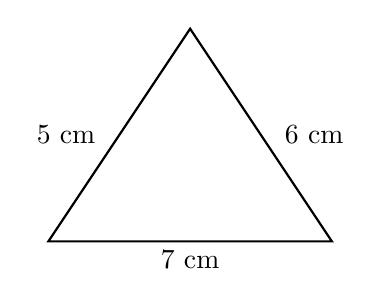
\begin{tikzpicture}[scale=0.9]
  \draw[thick] (0,0) -- (4,0) -- (2,3) -- cycle;
  \node[below] at (2,0) {$7$ cm};
  \node[left] at (0.8,1.5) {$5$ cm};
  \node[right] at (3.2,1.5) {$6$ cm};
\end{tikzpicture}
\end{center}
\end{questionText}
\choiceA{None}
\choiceB{Exactly one}
\choiceC{Exactly two}
\choiceD{Infinitely many}
\correctAnswer{B}
\explanation{Three side lengths that satisfy the triangle inequality (SSS) produce exactly one unique triangle. Check: $5 + 6 = 11 > 7$, $5 + 7 = 12 > 6$, $6 + 7 = 13 > 5$. All pass.}
\end{practiceQuestion}

\begin{practiceQuestion}{6-3-q28}{gmc}
\begin{questionText}
The four rectangles below all have the same perimeter of $16$ cm but different dimensions. What does this tell us?

\begin{center}
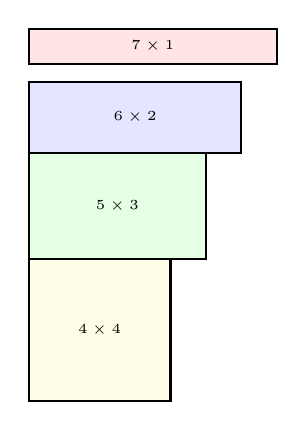
\begin{tikzpicture}[scale=0.45]
  \draw[thick,fill=red!10] (0,0) rectangle (7,1);
  \node at (3.5,0.5) {\tiny $7 \times 1$};
  \draw[thick,fill=blue!10] (0,-2.5) rectangle (6,-0.5);
  \node at (3,-1.5) {\tiny $6 \times 2$};
  \draw[thick,fill=green!10] (0,-5.5) rectangle (5,-2.5);
  \node at (2.5,-4) {\tiny $5 \times 3$};
  \draw[thick,fill=yellow!10] (0,-9.5) rectangle (4,-5.5);
  \node at (2,-7.5) {\tiny $4 \times 4$};
\end{tikzpicture}
\end{center}
\end{questionText}
\choiceA{A given perimeter determines exactly one rectangle}
\choiceB{A given perimeter allows more than one rectangle}
\choiceC{All rectangles with the same perimeter have the same area}
\choiceD{It is impossible for multiple rectangles to share a perimeter}
\correctAnswer{B}
\explanation{The four rectangles all have perimeter $16$ cm ($2(7+1) = 2(6+2) = 2(5+3) = 2(4+4) = 16$) but different shapes. A given perimeter allows many rectangles.}
\end{practiceQuestion}

\begin{practiceQuestion}{6-3-q29}{gsa}
\begin{questionText}
Look at the triangle below. Two angles are given. Can this triangle exist? If so, what is the third angle?

\begin{center}
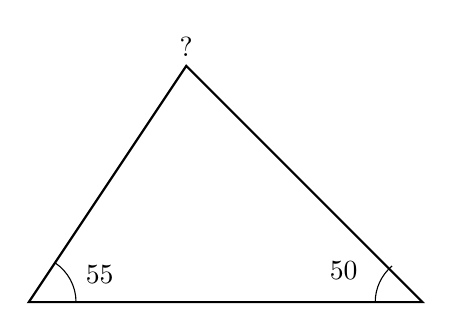
\begin{tikzpicture}[scale=1]
  \draw[thick] (0,0) -- (5,0) -- (2,3) -- cycle;
  \draw (0.6,0) arc[start angle=0,end angle=56,radius=0.6];
  \node at (0.9,0.35) {$55°$};
  \draw (4.4,0) arc[start angle=180,end angle=130,radius=0.6];
  \node at (4,0.4) {$50°$};
  \node[above] at (2,3) {$?$};
\end{tikzpicture}
\end{center}
\end{questionText}
\correctAnswer{Yes; the third angle is $75°$}
\explanation{$180° - 55° - 50° = 75°$. The angles sum to $180°$, so the triangle can exist. The third angle is $75°$.}
\end{practiceQuestion}

\begin{practiceQuestion}{6-3-q30}{gsa}
\begin{questionText}
The diagram below shows a triangle attempt with the given side lengths. Explain whether this triangle is possible using the triangle inequality.

\begin{center}
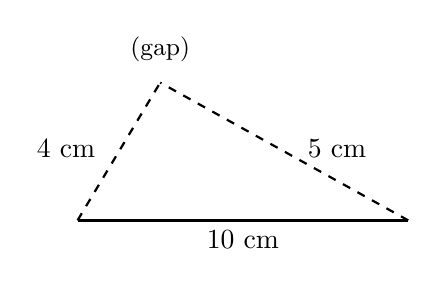
\begin{tikzpicture}[scale=0.7]
  \draw[thick] (0,0) -- (6,0);
  \draw[thick,dashed] (0,0) -- (1.5,2.5);
  \draw[thick,dashed] (6,0) -- (1.5,2.5);
  \node[below] at (3,0) {$10$ cm};
  \node[left] at (0.5,1.3) {$4$ cm};
  \node[right] at (4,1.3) {$5$ cm};
  \node[above] at (1.5,2.7) {\small (gap)};
\end{tikzpicture}
\end{center}
\end{questionText}
\correctAnswer{No, it is not possible}
\explanation{Check: $4 + 5 = 9 < 10$. The two shorter sides cannot connect across the base. The triangle inequality fails, so no triangle can be formed. The dashed lines with the gap illustrate that the sides don't meet.}
\end{practiceQuestion}
